% !Mode:: "TeX:UTF-8"
% -*-coding: utf-8 -*-

% Русский язык дополнительно настраивать не нужно.
% Убедитесь, что ваш редактор поддерживает UTF-8.
\documentclass{math-mech-sci}

% Название и авторы задаются при помощи специальных
% команд \deftitle и \defauthor. Специальные команды
% требуются для генерации корректной метаинформации в
% PDF-файле.
\newcommand{\X}{\mathsf X}
\renewcommand{\S}{\mathsf S}
\newcommand{\R}{\mathsf R}

\newcommand{\FPR}{\mathrm{FPR}}
\newcommand{\TPR}{\mathrm{TPR}}
\newcommand{\FARL}{\mathrm{FARL}}
\newcommand{\TARL}{\mathrm{TARL}}

\renewcommand{\geq}{\geqslant}

% Блоки в квадратных скобках опциональны, они предназначены
% для сносок на гранты, которыми поддержана работа.

\deftitle%
%  [\thanks{В квадратных скобках опционально,
%  кем и чем поддержана работа. Если никем и ничем,
%  убираем вместе со скобками.}]%
  {Подход к сравнению методов обнаружения
разладки}

\defauthor%
  {Шаповал Е.А.}%
  {СПбГУ, Санкт-Петербург}%
  {st063753@student.spbu.ru}
\defauthor%
  [\thanks{Работа поддержана грантом РНФ 23-21-00222.}]%
  {Голяндина Н.Э.}%
  {СПбГУ, Санкт-Петербург}%
  {n.golyandina@spbu.ru}

\begin{document}

\maketitle

\begin{abstract}
		Рассматривается задача обнаружения разладки во временных рядах с помощью функции разладки. Для сравнения методов обнаружения разладки предлагается подход, аналогичный использованию ROC кривых в
задачах классификации. Преимуществом подхода является то, что для сравнения методов на требуется задавать порог, при превышении которого метод сигнализирует о разладке. Особенности подхода продемонстрированы на примере. Показано, кривые, параметризованные порогом, где по оси X откладывается величина, обратная к средней длине интервала без сигнала о разладке в случае ее отсутствия, а по оси Y --- вероятность правильного обнаружения разладки с опозданием не больше заданного, является предпочтительной для сравнения. 
\end{abstract}

\section{Введение}

В работе рассматривается задача обнаружения разладки в сигнале при наблюдаемом зашумленном сигнале:  $\X_N=\S_N+\R_N$, где $\X_N$~--- наблюдаемый временной ряд длины $N$, $\S_N\in\mathbb R^N$~--- сигнал, $\R_N\in\mathbb R^N$~--- шум, т.е. стационарный случайный процесс.

Разладку можно определить, как некоторое изменение в структуре ряда. Приведем самый простой пример. Пусть $\S_N$ --- сигнал с общим членом
\begin{equation}\label{eq:mu}
s_n=\begin{cases}
 0,\quad n=1,\ldots,Q-1,\\
 \mu,\quad n=Q,\ldots,N,\\
\end{cases}
\end{equation}
$2<Q<N$, $\mu>0$, и $\R_N$ --- шум с общим членом $r_n\sim\mathcal N(0,\sigma^2)$, $\sigma>0$. Тогда временной ряд $\X_N=\S_N+\R_N$ можно рассмотреть как ряд, имеющий разладку в среднем случайного процесса.

Более сложный пример --- это разладка в частоте сигнала: 
\begin{equation}\label{eq:omega}
s_n=\begin{cases}
 A\cos(2\pi\omega_1n),\quad n=1,\ldots,Q-1,\\
 A\cos(2\pi\omega_2n+\varphi),\quad n=Q,\ldots,N,\\
\end{cases}
\end{equation}
$2<Q<N$, $A>0$, $|\omega_1-\omega_2|>\Delta>0$. 

Далее точку $Q$ будем называть \textit{точкой разладки}.

Для обнаружения разладки существует много разных методов, зависящих, в частности, от структуры сигнала и вида разладки [?,?]. Целью работы является построение способа сравнения методов обнаружения разладки, аналогичного использованию ROC-кривых в задачах классификации [?].

\section{Обнаружение разладки}
\subsection{Функция разладки}
Как правило, для обнаружения разладки строится функция разладки. % для временного ряда $\X_N$ как

\textbf{Определение 0.} Рассмотрим временной ряд $\X_N$, зафиксируем параметр $L=2,\ldots,N-1$~--- \textit{длина окна}. \textit{Функцией разладки} назовём отображение $h:\{L,L+1,\ldots,N\}\to\mathbb{R}_+$, у которого каждое значение $h_{i+L}$ зависит от отрезка временного ряда $(x_{i+1},\ldots,x_{i+L})$, $i=0,\ldots,N-L$. Назовём такой отрезок \textit{тестовым} и заметим, что функция разладки синхронизирована с его концом.

В качестве примера функции разладки для обнаружения разладки в среднем, если до этого среднее было равно нулю, рассмотрим
\begin{equation}\label{eq:h}
	h_{i+L}=\sum\limits_{j=i+1}^{i+L}x_j^2,
\end{equation}
$i=0,\ldots,N-L$.

% отображение $h:\{L,L+1,\ldots,N\}\to\mathbb R$, $L=2,\ldots,N-1$~--- параметр функции разладки,назовём его \textit{длиной окна}, $h_{i+L}$ зависит от значений временного ряда $x_i,\ldots,x_{i+L-1}$, $i=1,\ldots,N-L+1$, отрезок ряда, состоящий из этих значений назовём тестовым. То есть функция разладки синхронизирована с концом тестового отрезка. В качестве примера функции разладки можно рассмотреть $h_{i+L}=\sum\limits_{j=i}^{i+L-1}x_j^2$, $i=1,\ldots,N-L+1$.

На рис.~\ref{fig:x_mu_small} изображён временной ряд с разладкой в среднем случайного процесса с сигналом вида~\eqref{eq:mu}, где параметр $\mu=1$, а значение точки разладки $Q=200$,
На рис.~\ref{fig:e_mu_small} изображена его функция разладки вида~\eqref{eq:h}. Заметим, что после точки разладки $Q$ функция разладки $h$ начинает возрастать. Таким образом, можно её использовать как индикатор разладки во временном ряде.
\begin{figure}[h!]
	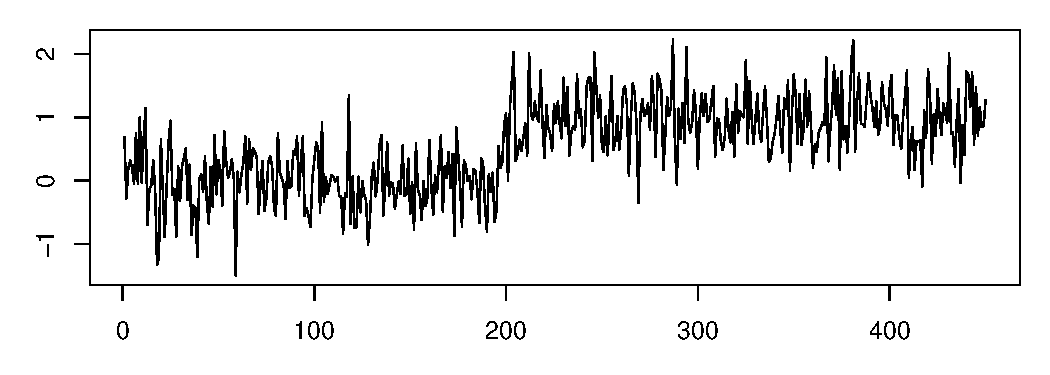
\includegraphics[width=\textwidth]{S_mu_small}\caption{Временной ряд $X_N$, $\mu=1$}\label{fig:x_mu_small}
\end{figure}
\begin{figure}
	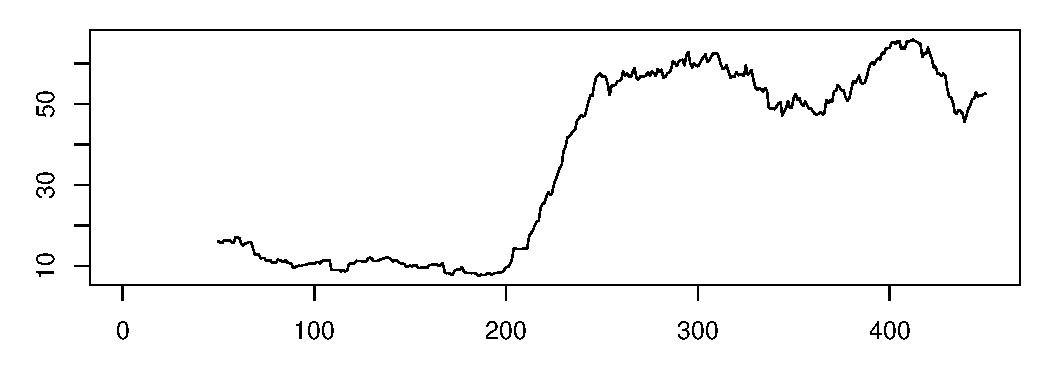
\includegraphics[width=\textwidth]{E_mu_small}\caption{Функция разладки ряда $X_N$, $\mu=1$}\label{fig:e_mu_small}
\end{figure}

\subsection{Оценка точки разладки}
Введем некоторое число $\theta >0$, далее будем называть это число \textit{порогом}. Пусть $h$~--- функция разладки ряда $X_N$, оценим точку разладки $Q$ как
\begin{equation}
\widehat Q(h,\theta):=\min\{i\in\{L,L+1,\ldots,N\}:h_i>\theta\}.
\end{equation}

Выделим две задачи, которые нужно решить для определения точки разладки указанным способом: выбор вида функции разладки и выбор значения порога $\theta$. 
%\begin{itemize}
%	\item Выбор вида функ
%	\item
%\end{itemize}

Для оценки качества работы алгоритма по обнаружению точки разладки зафиксируем натуральное $k$, назовём его \textit{допустимым временем запаздывания}. Пусть $\widehat Q$~--- оценка $Q$. Определим следующие виды срабатываний:
\begin{itemize}
	\item $\widehat Q\in [Q,Q+k]$~--- оценка $Q$ правильная, правильное срабатывание (true alarm),
	\item $\widehat Q<Q$~--- ложное срабатывание (false alarm),
	\item $\widehat Q>Q+k$~--- срабатывание с запаздыванием (delay).
\end{itemize}

Для оценки false alarm и true alarm выделим два подхода: через вероятности и <<в среднем>>. Для оценки вероятности false alarm будем использовать
%\begin{itemize}
%	\item Вероятностный,
	\begin{equation}
	\FPR:=\Prob(\widehat Q<Q),
	\end{equation}
	обратим внимание, что $\FPR$ зависит от значения $Q$. 

Оценка вероятности true alarm может быть записана как
	\begin{equation}
		\TPR:=\Prob(\widehat Q\in[Q,Q+k]\mid \widehat Q\geq Q).
	\end{equation}
	
	%\item В среднем, $\FARL:=\mathsf E\widehat Q$ на ряде без разладки, $\TARL:=\mathsf E (\widehat Q\mid \widehat Q\geq Q)$.
	%\item $\widehat Q>Q+k$~--- срабатывание с запаздыванием (delay)
%\end{itemize}

Учитывая что $\FPR = \FPR(Q,h,\theta)$ и $\TPR= \TPR(k,h,\theta)$ --- монотонно невозрастающие функции по $\theta$, можно выделить две постановки задачи.
\begin{itemize}
	\item Максимизировать $\TPR$ при условии $\FPR<\alpha$, где $\alpha\in(0,1)$ --- максимально допустимая вероятность false alarm за время $Q$; эта постановка задачи стандартная и в ней легче получать теоретические результаты.
	\item Минимизировать $\FPR$ при условии $\TPR>\gamma$, где $\gamma\in(0,1)$ --- вероятность своевременного обнаружения разладки; такая постановка задачи ближе к практике, но в ней нужно конкретизировать вид разладки.
\end{itemize}

	В подходе <<в среднем>> вычисляют
	\begin{equation}
	\FARL:=\mathsf E\widehat Q
	\end{equation}
	для ряда без разладки, а для ряда с разладкой ---
	\begin{equation}
		\TARL:=\mathsf E (\widehat Q\mid \widehat Q\geq Q).
	\end{equation}

Аналогично подходам через вероятности можно сформулировать задачи, используя $\FARL$ и/или $\TARL$. Выбор порога в обеих постановках~--- сложная задача.

\subsection{Примеры постановок задач}
Опишем пример первой постановки задачи, с условием $\FPR<\alpha$. Будем рассматривать временной ряд с сигналом вида~\eqref{eq:mu}, для функции разладки вида~\eqref{eq:h} аппроксимацию значений $\FPR$ и $\FARL$ для больших $Q$ можно найти аналитически (Noonan, Zhigljavsky, 2020). Затем по найденным аппроксимациям можно находить порог $\theta$. Данный пример можно обобщить до следующего вида. Общий член сигнала $\S_N$ имеет вид
\begin{equation}
	s_n=\begin{cases}
		u_n,\quad n=1,\ldots,Q-1,\\
		u_n+\mu,\quad n=Q,\ldots,N,\\
	\end{cases}
\end{equation}
	$\mu>0$, временной ряд $\mathsf U_N=(u_1,u_2,\ldots,u_N)$ выделяется некоторым методом, например, методом анализа сингулярного спектра (SSA) [ссылка], а далее разработанная теория применяется к остатку.
	
	Пример второй постановки задачи рассмотрен в [ссылка на мою работу], для сигнала вида~\eqref{eq:omega}, функция разладки строилась на основе метода анализа сингулярного спектра (SSA). В работе был теоретически найден порог, при котором в наихудшем по $\omega_2$ и $\varphi$ случае выполняется неравенство $\TPR>\gamma$.
	
\section{Способ сравнения методов обнаружения разладки}
	Рассмотрим два вида аналога ROC-кривых для определения качества метода обнаружения разладки. 

	\textbf{Определение 0.} Рассмотрим функцию разладки $h$ временного ряд $\X_N$ и набор порогов $\Theta\subset\mathbb R$. Назовем \textit{$\FPR-\TPR$ кривой} параметрически заданную кривую $\{(x,y)\in\mathbb R^2:x=\FPR(Q,h,\theta),y=\TPR(k,h,\theta),\theta\in\Theta\}$ и \textit{$\FARL-\TPR$ кривой} параметрически заданную кривую $\{(x,y)\in\mathbb R^2:x=1/\FARL(h,\theta),y=\TPR(k,h,\theta),\theta\in\Theta\}$.
%$\FPR(h,\theta)$~--- значение $\FPR$ при его подсчёте с помощью функции $h$ по порогу $\theta$, аналогично с $\TPR$. 

Обе кривые определены так, что чем выше лежит кривая, тем лучше работает метод обнаружения разладки. Введенные кривые позволяют сравнивать методы для всех множества порогов, без вычисления конкретного.
	
Для демонстрации использования введенных кривых рассмотрим пример с разладкой в среднем и введем два вида функции разладки. Сначала определим функцию разладки с весами.
	
	\textbf{Определение 0.} Рассмотрим временной ряд $\X_N$, зафиксируем параметр $L$, рассмотрим \textit{вектор весов} $w=(w_1,\ldots,w_L)\in\mathbb R^L$. \textit{Функцией разладки с весами} $w$ назовём функцию
	\begin{equation}
		h_{i+L}:=\sum\limits_{j=1}^Lw_jx_{i+j}^2,
	\end{equation}
	$i=0,\ldots,N-L$.

Рассмотрим функции разладки с двумя видами весов:
	\begin{itemize}
		\item стандартная (unweighted), $h_{i+L}^0:=\sum\limits_{j=1}^Lx_{i+j}^2$, $w^0=(1,1,\ldots,1)$,
		\item взвешенная (weighted), $h_{i+L}^{(k)}:=\sum\limits_{j=k}^Lx_{i+j}^2$, $w^{(k)}=(0,\ldots,0,\underbrace{1,\ldots,1}_{k})$.
	\end{itemize}


\subsection{Численные эксперименты}
В качестве примера будем рассматривать временной ряд с разладкой в среднем, то есть сигнал вида~\eqref{eq:mu}, параметры $Q=60$ и $Q =150$, $\sigma=1$, $L=50$, $k=10$. Оценки $\FPR$, $\TPR$ и $\FARL$ будем проводить по выборке объёма $n=100$.

Сначала построим графики для случая без разладки, $\mu=0$, для разных значений $Q$ для того, чтобы относительно него оценивать эффективность метода обнаружения разладки. На рис.~\ref{fig:def} видно, что для различных $Q$ получаем различные исходные оценки даже при отсутствии разладки. Более того, получаем разную упорядоченность методов даже при отсутствии разладки.

\begin{figure}[h]
	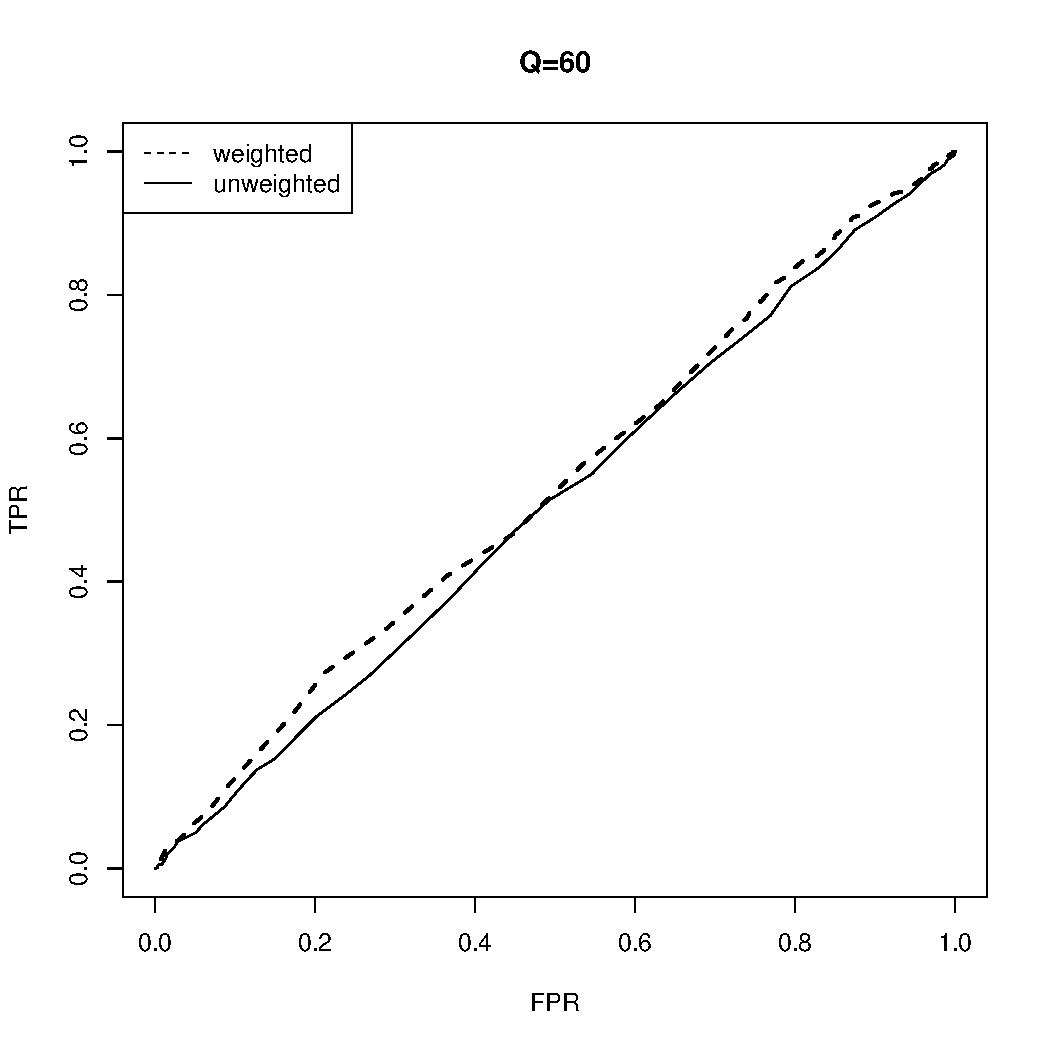
\includegraphics[width=0.45\textwidth]{def_10}
	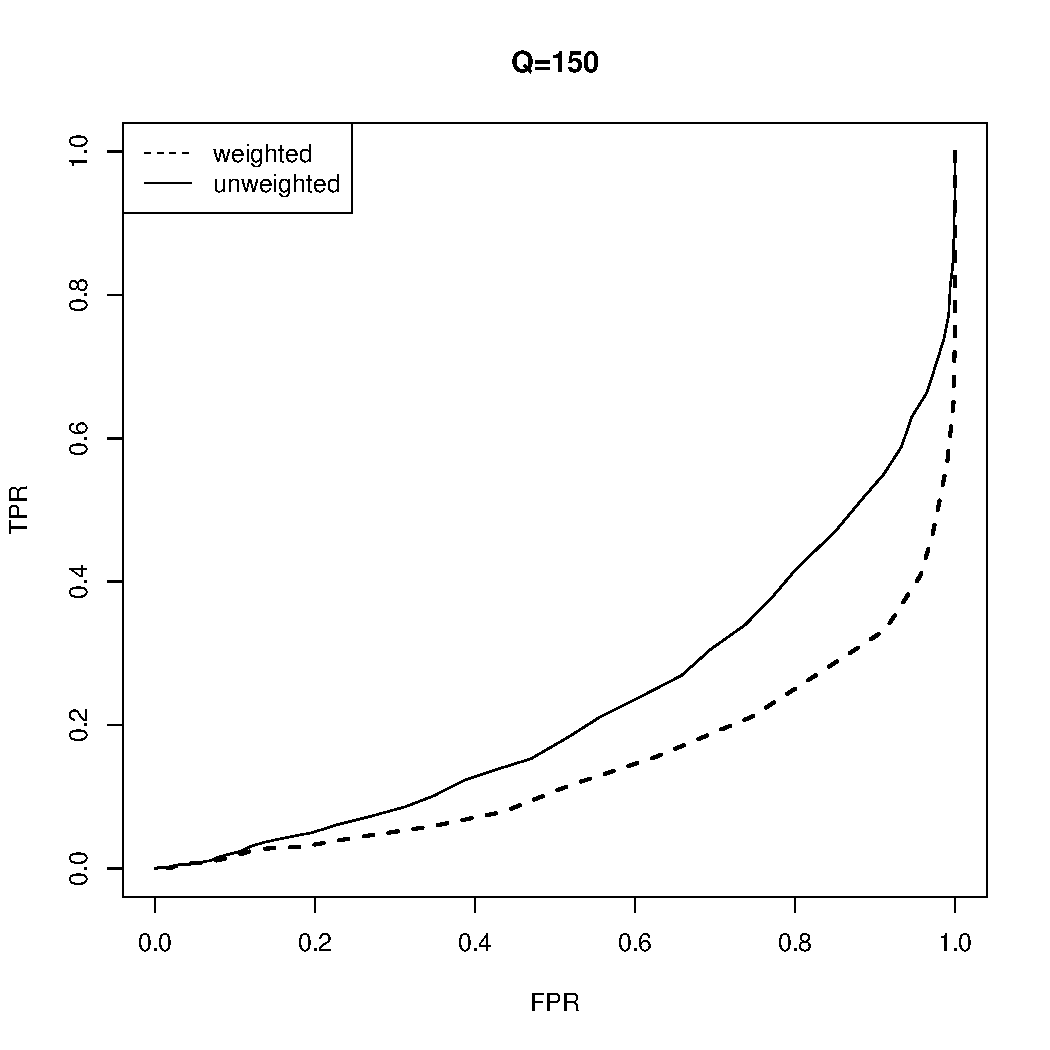
\includegraphics[width=0.45\textwidth]{def_100}\caption{$\mathrm{FPR}-\mathrm{TPR}$ кривые, $\mu=0$, $Q=60$ (слева) и $150$ (справа)}\label{fig:def}
\end{figure}

Теперь рассмотрим случай с маленькой разладкой ($\mu=0.5$). На рис.\ref{fig:ex} видно, что для $Q=50$ взвешенный вариант функции разладки лучше, а для $Q=150$ лучше стандартный. То есть результат сравнения методов зависит от значения $Q$.


\begin{figure}[h]
	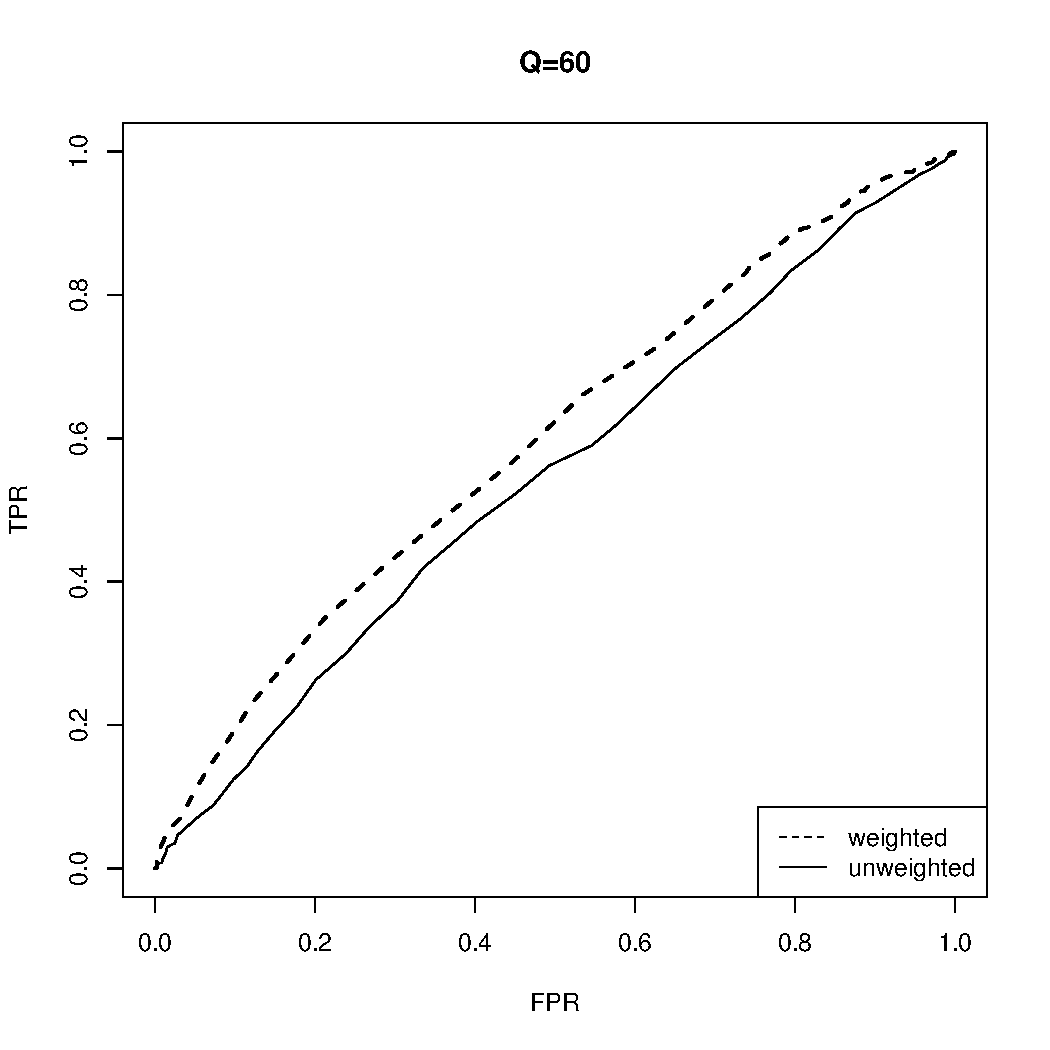
\includegraphics[width=0.45\textwidth]{ex_10}
	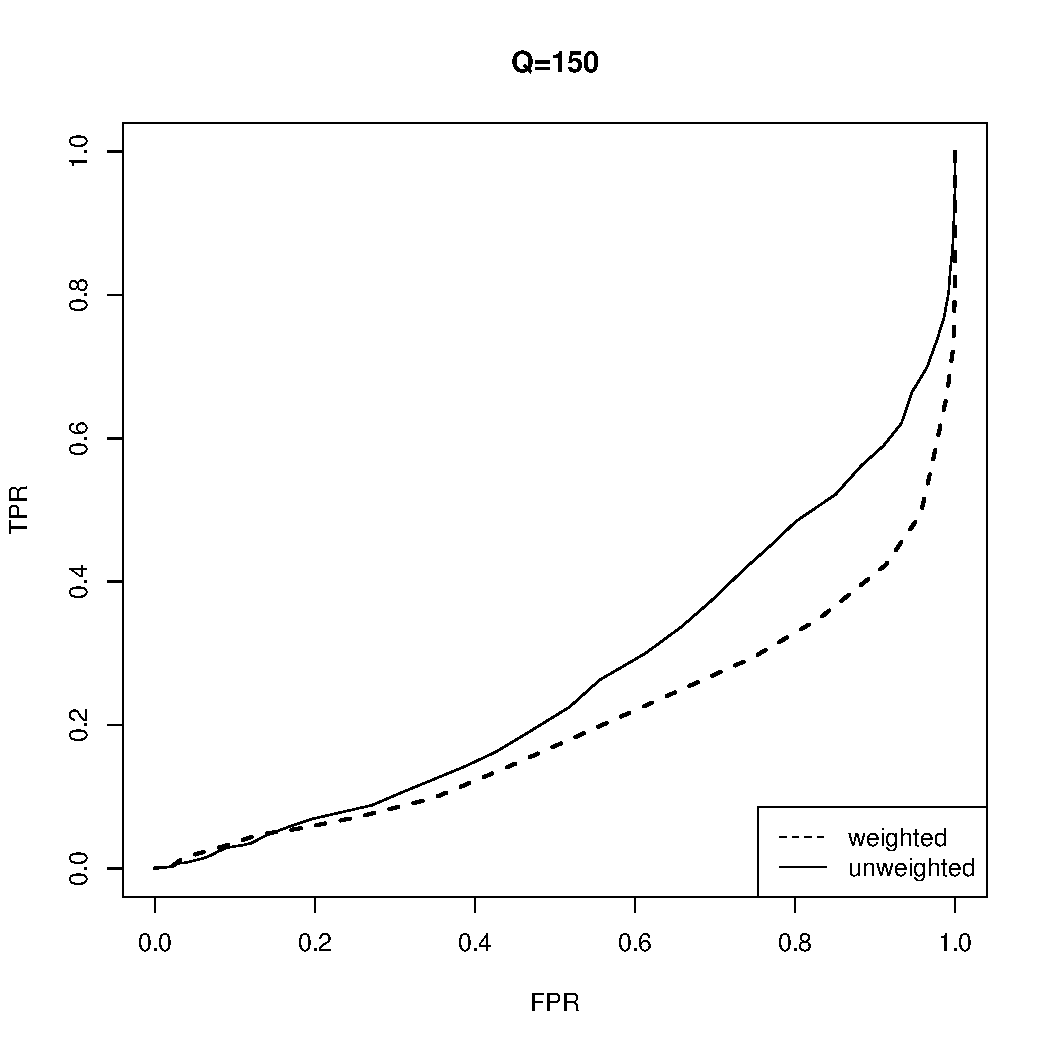
\includegraphics[width=0.45\textwidth]{ex_100}\caption{$\mathrm{FPR}-\mathrm{TPR}$ кривые, $\mu=0.5$, $Q=60$ (слева) и $150$ (справа)}\label{fig:ex}
\end{figure}

Для того чтобы результат сравнения методов не зависел от $Q$, вместо значения $\FPR$ по оси $X$ будем откладывать значение $1/\FARL$, т.е. рассмотрим $\FARL-\TPR$ кривые. Построим их для двух примеров с разной величиной разладки, $\mu=0.5$ и $\mu =2$. На рис.~\ref{fig:arl} изображены пары $\FARL-\TPR$ кривых. По $\FARL-\TPR$ кривым можно установить, что для примера с $\mu=0.5$ стандартный вариант функции разладки лучше взвешенного, а для примера с большим $\mu=2$ лучше взвешенный вариант.

\begin{figure}
	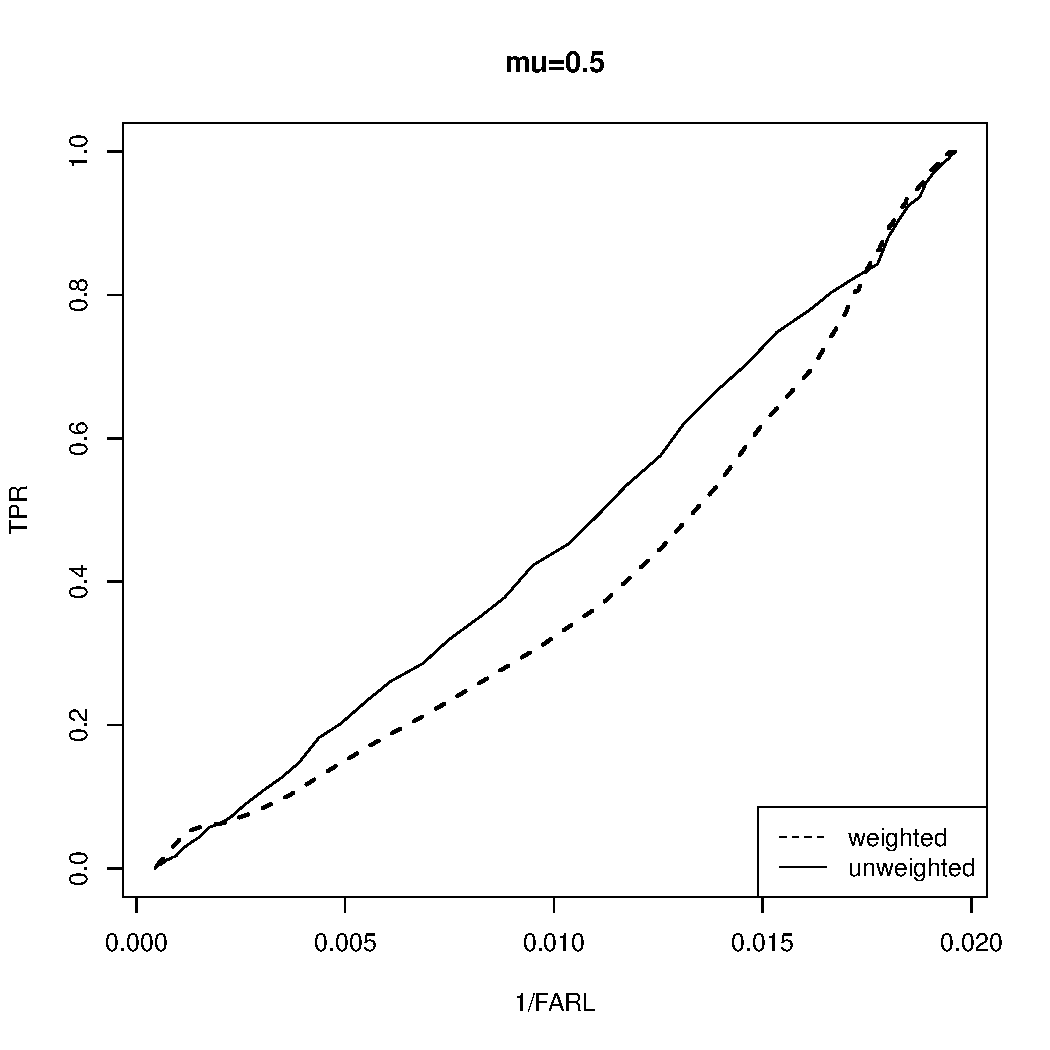
\includegraphics[width=0.45\textwidth]{arl_0.5}
	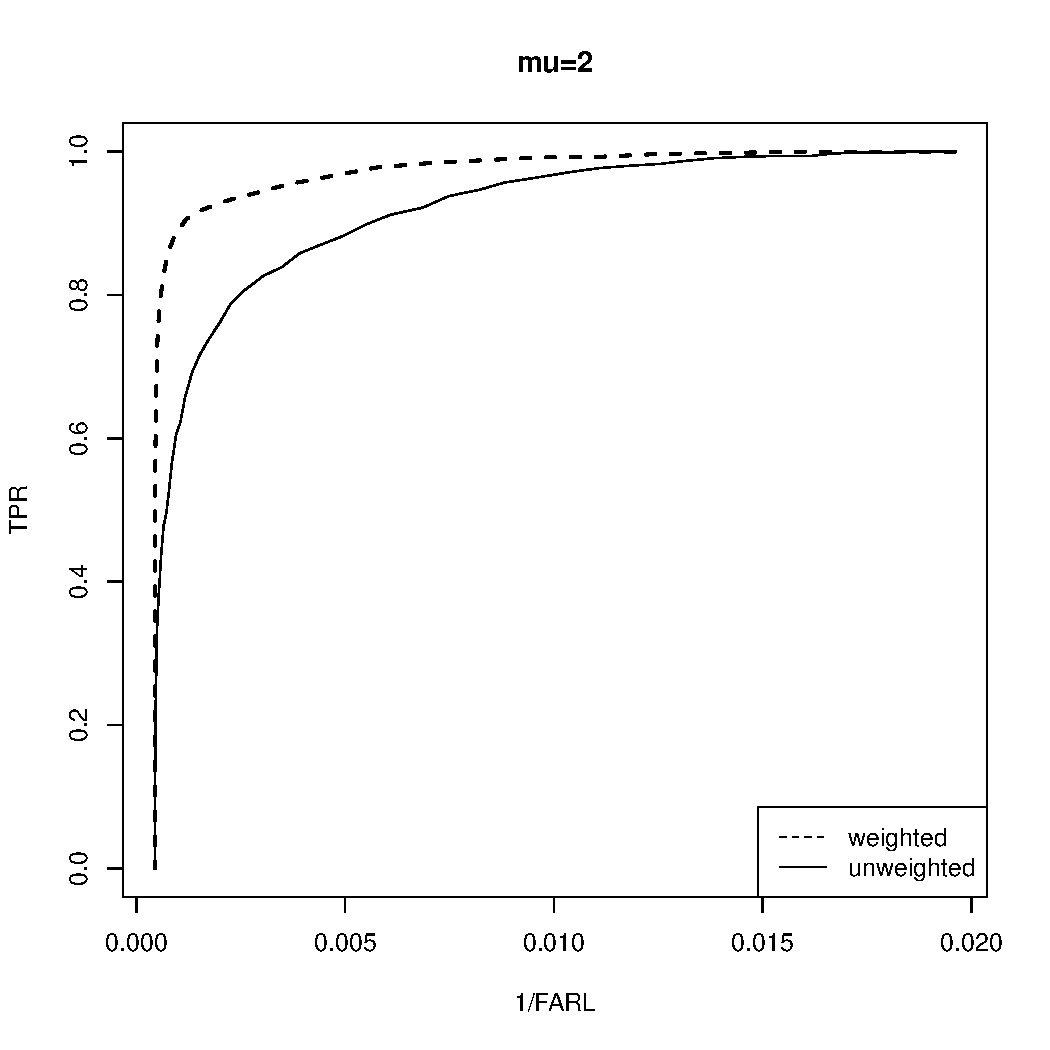
\includegraphics[width=0.45\textwidth]{arl_2}\caption{$\mathrm{FARL}-\mathrm{TPR}$ кривые, $Q=60$, $\mu=0.5,2$}\label{fig:arl}
\end{figure}

\section{Заключение}
	Для сравнения способов обнаружения разладки был разработан
подход, аналогичный использованию ROC кривых в
задачах классификации. Преимуществом подхода является то, что для сравнения методов не требуется выполнять сложную и часто не полностью теоретически обоснованную процедуру определения подходящего порога. Особенности подхода были продемонстрирован на примере разладки в среднем гауссовского процесса. В результате, были показаны недостатки $\FPR-\TPR$ кривых, вызванные тем, что вероятность $\FPR$ зависит от длины промежутка, на котором измеряется false alarm.  В свою очередь, $\FARL-\TPR$ кривые, где вероятность $\FPR$ заменяется на величину, обратную к средней длине интервала без false alarm, не обладает таким недостатком, поэтому сравнение методов обнаружения разладки по $\FARL-\TPR$ кривым представляется более предпочтительным.

\begin{thebibliography}{8}

\bibitem{medvedev2011} Медведев О. Use case: отладка реализации RISC
  процессора для FPGA // % Материалы 2-й межвузовской научной
  конференции по проблемам информатики<<СПИСОК-2011>>. --- % 2011. ---
  С. 7--12.
  \href{http://math-science.math.spbu.ru/txt/math-science-2011.pdf}{http://math-science.math.spbu.ru/txt/math-science-2011.pdf}

\end{thebibliography}

\end{document}
